\chapter{Herramientas Empleadas}\label{cap:herramientas}

En este capítulo se explican las herramientas, librerías y APIs que se han utilizado en el desarrollo de AdaptaMaterialEscolar 2.0. En la Sección \ref{sec:Figma} se introduce la herramienta Figma que se ha usado para realizar el diseño de la aplicación. En la Sección \ref{sec:React} se presenta la libreria React que se ha empleado para implementar las interfaces de usuario de la aplicación. En la Sección \ref{sec:tailwind} se explica el framework Tailwind CSS, que se ha usado para personalizar el estilo de las páginas y los distintos elementos que las componen. En la Sección \ref{sec:Slate} se expone el framework Slate que se usa para definir el editor.

\section{Figma}\label{sec:Figma}
Figma\footnote{\url{https://www.figma.com/}} es una herramienta web de diseño y prototipado de interfaces de usuario que ofrece una amplia gama de herramientas y recursos para crear diseños de alta calidad de manera eficiente y efectiva. Esta herramienta es especialmente útil para el diseño de aplicaciones móviles y web debido a su funcionalidad de colaboración en tiempo real y la facilidad de acceso.
\\

Hemos empleado Figma porque nos permite crear diseños de alta fidelidad con facilidad y rapidez. Además, Figma también cuenta con una amplia variedad de recursos de diseño, como kits de interfaz de usuario y plantillas, lo que facilita aún más la creación de diseños profesionales. A eso debemos sumarle su exportabilidad, que nos permite extraer css de los diseños implementados en Figma.
\\

En definitiva, Figma es una herramienta muy útil y efectiva para temas de diseño, debido a ello todo el diseño final de la aplicación ha sido realizado en Figma, tal y como se explicará en la Seccion \ref{subsec:DisenyoFinal}.

\section{React}\label{sec:React}
React\footnote{\url{https://es.reactjs.org/}} es una librería de JavaScript que se utiliza para crear interfaces de usuario interactivas y dinámicas en aplicaciones web. Fue desarrollada por Facebook y es una de las herramientas más populares para construir aplicaciones web modernas. En nuestra aplicación, hemos utilizado React para implementar las interfaces de usuario.

React utiliza un enfoque basado en componentes para construir interfaces de usuario, lo que significa que cada parte de la interfaz de usuario se representa como un componente. Dichos componentes son reutilizables y están diseñados para ser simples, fáciles de mantener y declarativos, es decir, describe qué se quiere hacer y no cómo hacerlo. Otras ventajas que ofrece son:

\begin{itemize}
  \item \textbf{Mayor eficiencia}: React utiliza un enfoque llamado ``reconciliación virtual'' para actualizar la interfaz de usuario de manera eficiente y minimizar el impacto en el rendimiento. Este enfoque se basa en la comparación de los estados previos y actuales de los componentes, permitiendo actualizar solo las partes necesarias de la interfaz.
  \item \textbf{Facilidad de mantenimiento}: Como se ha mencionado anteriormente los componentes de React son simples y declarativos, lo que hace que sea más fácil mantener y actualizar una aplicación web construida con React.
  \item \textbf{Biblioteca de componentes}: React tiene una gran biblioteca de componentes disponibles para su uso, lo que permite a los desarrolladores construir aplicaciones web complejas con facilidad.
\end{itemize}

Para representar las interfaces de usuario en React se utiliza una extensión de sintaxis llamada JSX que permite escribir HTML en JavaScript, lo que hace que el código sea más legible y fácil de entender. En JSX los elementos de la interfaz de usuario se definen como etiquetas HTML dentro del código JavaScript. En la Figura \ref{JSX} se muestra un ejemplo de un componente usando JSX y en la Figura \ref{SJSX} se encuentra la misma funcionalidad pero sin JSX.

\begin{figure}[ht!]

  \begin{subfigure}{\textwidth}
    \centering
    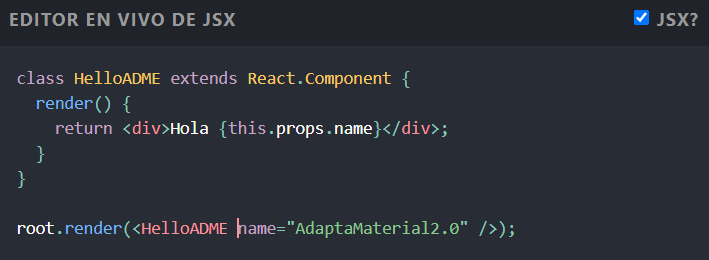
\includegraphics[width=0.6\textwidth]{Herraientas_Empleadas/ReactJSX.PNG}
    \caption{Componente con JSX.}
    \label{JSX}
  \end{subfigure}

  \begin{subfigure}{\textwidth}
    \centering
    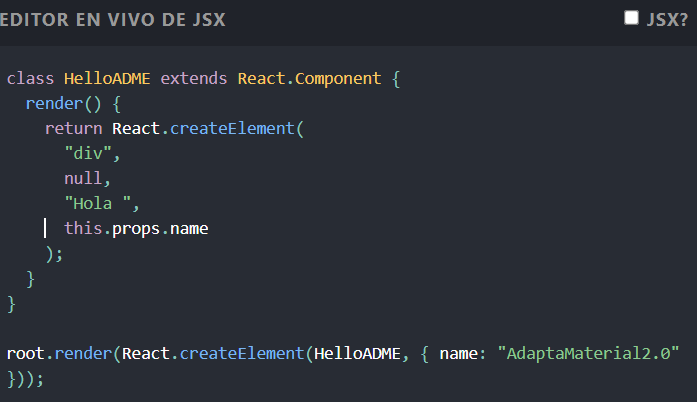
\includegraphics[width=0.6\textwidth]{Herraientas_Empleadas/ReactSinJSX.PNG}
    \caption{Componente sin JSX.}
    \label{SJSX}
  \end{subfigure}
  \caption{Componentes React}
  \label{fig:react}
\end{figure}

En los componentes de React se utiliza Tailwind CSS, una librería de estilos CSS, para la construcción rápida de interfaces de usuario sin tener que escribir CSS personalizado para cada elemento. En la siguiente subsección se hablará de ella.



\section{Tailwind CSS}\label{sec:tailwind}
Tailwind CSS\footnote{\url{https://tailwindcss.com/}} es un framework CSS que permite aplicar estilos predefinidos directamente en el HTML sin tener que crear y manejar archivos CSS propios para conseguir un estilo concreto. Hemos decidido utilizar este framework porque facilita la labor de dar estilo al HTML de la página, debido a que no tenemos que pensar en qué clases o identificadores dar a los elementos HTML y, por lo general, tampoco necesitamos gestionar un archivo CSS por cada página o componente de React. Otra de las razones por las que hemos escogido este framework frente a otros muy parecidos, como Bootstrap\footnote{\url{https://getbootstrap.com/}}, es la facilidad que ofrece para personalizarlo y adaptarlo a nuestras necesidades. En el caso de Bootstrap, necesitas utilizar SASS o crear tus propios archivos CSS para poder personalizar el estilo, mientras que en Tailwind CSS modificando un archivo de configuración puedes personalizar/añadir colores, añadir distintos tipos de fuente de texto, añadir distintos tamaños de letra, etc. Otras ventajas que ofrece son:
\begin{itemize}
  \item \textbf{Rendimiento}: Tailwind elimina automáticamente todo el CSS que no se utilice a la hora de desplegar en producción la aplicación, consiguiendo que el paquete de CSS que se envía al cliente sea lo más pequeño posible.
  \item \textbf{Diseño responsive}: Permite aplicar distintos estilos dependiendo del tamaño de la ventana sin necesidad de pelearse con \textit{media queries}\footnote{\url{https://developer.mozilla.org/en-US/docs/Web/CSS/Media_Queries/Using_media_queries}} de CSS.
  \item \textbf{Reutilización}: Tailwind permite reutilizar conjuntos de utilidades que se repitan mucho definiendo una clase CSS propia que los aplique todos. Aun así, nosotros no utilizaremos, principalmente, el método que ofrece Tailwind para reutilizar estilos, ya que podemos conseguir el mismo resultado creando un componente de React, con la ventaja de poder añadir lógica de JavaScript.
\end{itemize}

% TODO: Añadir ejemplos de uso

\section{Slate}\label{sec:Slate}
Slate\footnote{\url{https://docs.slatejs.org/}} es un framework de JavaScript de código abierto que tiene como finalidad la creación de editores de texto personalizados ``What You See Is What You Get'' (WYSIWYG). Es la herramienta ideal para este proyecto, el cual busca construir un editor de texto de alta calidad capaz de realizar diversos tipos de adaptación curricular.

A diferencia de las bibliotecas de edición de texto convencionales, Slate utiliza una estructura de árbol de datos jerárquica para representar el contenido editable. En lugar de usar la estructura lineal tradicional, la estructura de árbol permite una mayor flexibilidad y personalización en la creación y edición de contenido.

El árbol de Slate está compuesto por nodos que representan diferentes tipos de contenido, como texto sin formato, texto con formato, imágenes, videos y más. El nodo principal del árbol es el nodo documento, que es el contenedor de todos los demás nodos. Cada nodo hijo del nodo documento puede ser un nodo hoja o un nodo de elemento.

Los nodos de hoja contienen el contenido de texto real, mientras que los nodos de elemento contienen información sobre el formato, el estilo y otras propiedades del contenido. Cada nodo de elemento puede tener varios nodos secundarios, y estos nodos pueden ser de cualquier tipo que el desarrollador desee definir. Por ejemplo, un nodo de elemento podría representar un párrafo, una lista, etc. Podemos ver un ejemplo de esta estructura en la Figura \ref{fig:arbolSlate}.

\begin{figure}[ht!]
  \centering
  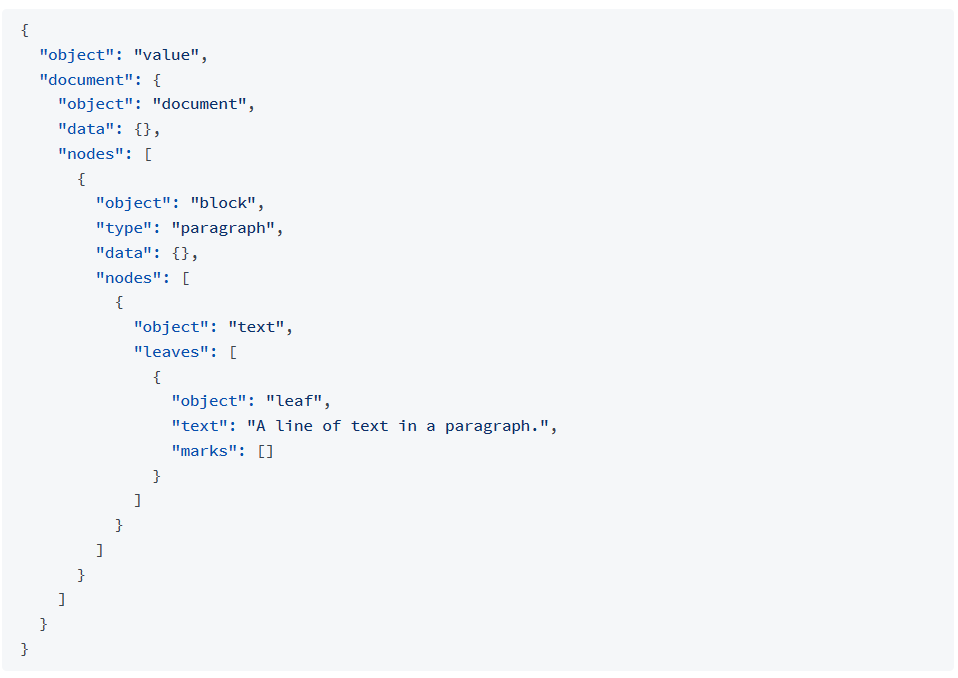
\includegraphics[width=0.7\textwidth]{Herraientas_Empleadas/ArbolSlate.png}
  \caption{Ejemplo de árbol de Slate}
  \label{fig:arbolSlate}
\end{figure}

Cada nodo en el árbol de Slate también puede tener una serie de propiedades que describen el contenido y su estilo. Estas propiedades se almacenan en un objeto llamado ``props''. Además, Slate proporciona una API para manipular el contenido de manera más efectiva.

Las principales características de Slate incluyen:

\begin{itemize}
  \item \textbf{Personalización}: La biblioteca permite a los desarrolladores personalizar el editor de texto según sus necesidades, lo que significa que pueden definir sus propios tipos de nodos y componentes de renderizado.
  \item \textbf{Flexibilidad}: Al ser una biblioteca de JavaScript, Slate es altamente flexible y puede integrarse fácilmente con otras bibliotecas y marcos como React.
  \item \textbf{Rendimiento}: La estructura de árbol de datos utilizada por Slate permite que la biblioteca realice actualizaciones eficientes del DOM, lo que resulta en un editor de texto rápido y fluido.
  \item \textbf{Soporte de complementos}: Los complementos de Slate son módulos que proporcionan una funcionalidad adicional al editor de texto. Estos complementos pueden personalizarse y utilizarse según las necesidades del desarrollador.
  \item \textbf{Compatibilidad multiplataforma}: Slate es compatible con una amplia gama de navegadores y plataformas.
\end{itemize}

Slate es utilizado por variedad de aplicaciones web como, por ejemplo:
\begin{itemize}
  \item \textbf{Discord}: Utiliza Slate para sus canales de comunicación para colaborar y compartir.
  \item \textbf{Eraser}: Una aplicación web de borrador de fondos que utiliza Slate para permitir a los usuarios escribir y editar el texto en su sitio web.
  \item \textbf{GitBook}: Es una plataforma de creación y publicación de libros electrónicos que utiliza Slate como editor de texto para que los autores puedan escribir y editar sus libros.
\end{itemize}